\documentclass{beamer}

\usepackage{lmodern}
\usepackage[french]{babel}
\usepackage[utf8]{inputenc}
\usepackage[T1]{fontenc}

\usetheme{Warsaw}
\setbeamerfont{page number in head/foot}{size=\large}
\setbeamertemplate{footline}[frame number]
\beamertemplatenavigationsymbolsempty

\title{Détection des ondes gravitationnelles}
\begin{document}

\begin{frame}
	\titlepage
\end{frame}

\begin{frame}
	\frametitle{Plan de l'exposé}
	\begin{enumerate}[I.]
		\item Les ondes gravitationnelles
		\item Présentation de l'interféromètre de Michelson
		\item Les Lasers
	\end{enumerate}
\end{frame}


\section{Présentation du Michelson}

\begin{frame}
	\frametitle{Interféromètre de Michelson}
	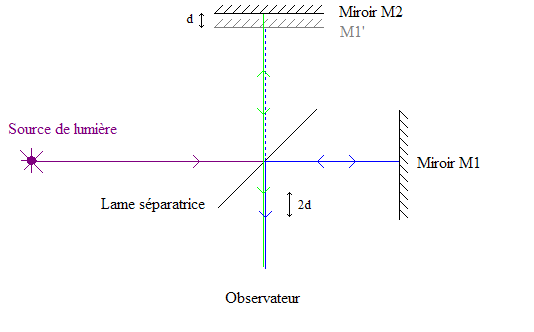
\includegraphics[scale=0.5]{Docs/interferometre_michelson.png}
\end{frame}


\section{Présentation des interféromètres LIGO / VIRGO}
\begin{frame}
	\frametitle{L'interféromètre VIRGO}
	\begin{columns}
		\begin{column}{0.5\textwidth}
			\small
			\begin{enumerate}[-]
				\item 2 bras de 4km de long parfaitement horizontaux (Sous Vide)
				\item Système complètement isolé de l'exterieur
			\end{enumerate}
		\end{column}
		\begin{column}{0.5\textwidth}
			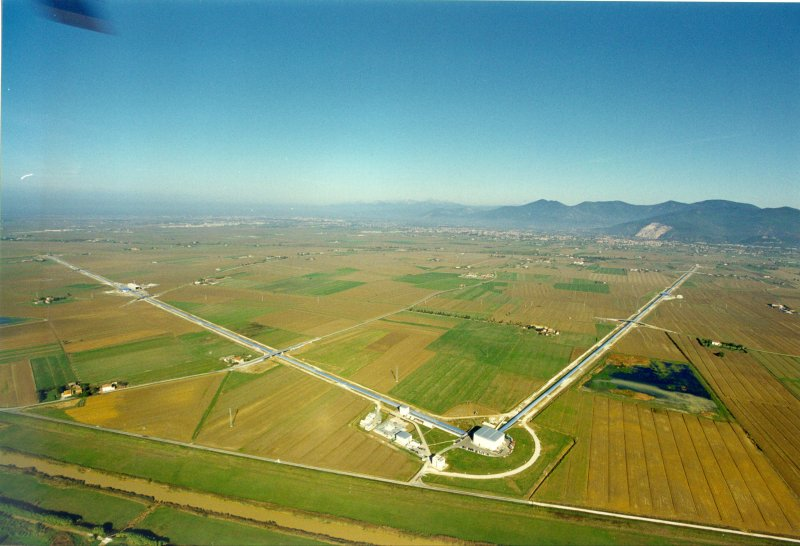
\includegraphics[scale=.5]{Docs/virgoview.png}
		\end{column}
	\end{columns}
	\bigskip
	2 interféromètres: VIRGO (Italie) et LIGO(Hanford(Washington) / Livinston (Louisianne))
\end{frame}
\section{LASER}


\begin{frame}
	\frametitle{Système injection}
	2 Lasers: Un laser maître et un laser esclave
	\break

	On injecte un rayonnement laser dans la cavité du second laser pour faire change son gain et modifier la fréquence d'émission du second laser.
\end{frame}

\begin{frame}
	\frametitle{Le laser de LIGO}
	Fonctionne en quatre étapes
	\begin{enumerate}[1.]
		\item Emission du laser Maître par une photodiode
		\item Emission du laser Esclave
		\item Première amplification
		\item Seconde amplification 
	\end{enumerate}
\end{frame}
\end{document}
